\chapter{Una torre más o menos medieval -- III}

\lettrine[ante=\raisebox{-1.5ex}{\Large ---},lines=2]{Y}{a tenemos}
ladrillos y pisos ---recapituló Antonia---; ahora definamos la torre.

Cecilia entendió inmediatamente que ese plural aludía a ella.

\section{La torre}

Con la mirada vuelta hacia el monitor, y la imaginación puesta en el
dibujo original de la torre que le había mostrado Antonia, Cecilia
pensaba: <<Bien, esto es bastante fácil: una torre no es más que una
colección de pisos colocados uno encima del otro. Pero no te apures,
Cecilia>> ---se dijo a sí misma---; <<primero lo primero: escribamos
el esqueleto del módulo torre>>:

\begin{lstlisting}
module torre ( ) {

}
\end{lstlisting}
  % \end{minipage}\hfill
  % \begin{minipage}[]{.5\textwidth}
  %     \centering
  %     \includegraphics[width=.6\textwidth]{imagenes/vacio}
  %   \end{minipage}
  % \end{center}

<<Excelente>> ---Cecilia trató de darse ánimos para
con\-ti\-nuar---. <<¿Qué parámetros definen una torre? Claramente, su
altura. ¡Ah! También la cantidad de pisos que tenga>>.

Si bien se obligó a seguir pensando, sólo pudo concluir que los demás
parámetros que se le ocurrían pertenecían a cada piso: radio, espesor
de las paredes, etc.

    \begin{lstlisting}
module torre (
  altura,
  n_pisos) {

}
    \end{lstlisting}


    <<Muy bien; ahora supongo que debo crear un bucle que repita, para
    cada valor de \texttt{n\_pisos}, un piso trasladado hacia
    arriba. Pero, ¿cuánto debo trasladarlos?>> ---Ce\-ci\-lia pensó un
    mo\-men\-to---. <<¡Claro! Si tengo que repartir la \texttt{altura}
    entre \texttt{n\_pisos}, cada piso medirá
    $\frac{\text{altura}}{\text{n\_pisos}}$ de alto>>:

    \begin{lstlisting}
module torre (
  altura,
  n_pisos) {
  alto_piso=altura/n_pisos;
  for (i=[0:n_pisos]){
    z=i*alto_piso;
    translate([0,0,z])
      piso(40,
           alto_piso,
           5,
           20);
  }
}
    \end{lstlisting}


    Cecilia no pudo evitar cierto orgullo mientras releía su texto. En
    la línea 4 calculaba la altura de cada uno de los pisos. En la
    definición del bucle de la línea 5, la variable i recorría cada
    uno de ellos. En la línea 6 calculaba la altura \texttt{z} que
    debían ser trasladados hacia arriba, y enseguida los creaba y
    trasladaba.

    ---Cecilia ---Antonia interrumpió sus pensamientos con un tono que
    hizo que su compañera intuyera la inminencia de un
    pro\-ble\-ma---: ¿Por qué hiciste variar i desde 0 hasta
    \texttt{n\_pisos}?

    Cecilia respondió con sencillez:

    ---Porque quería que el primer piso estuviera... bueno... en el
    `piso'; para eso necesitaba que el primer valor de \texttt{z}
    fuera igual a 0, lo cual sólo podía conseguir haciendo que
    \texttt{i} comenzara en ese valor en lugar de 1 ---Cecilia no
    podía ver ninguna fisura en su razonamiento.

    Antonia replicó suavemente:

    ---En eso estoy completamente de acuerdo; lo que cuestiono es la
    cota superior...

  Cecilia volvió a mirar, extrañada, el texto: ¿qué problema podía
  haber en usar \texttt{n\_pisos} como máximo? ¿No era precisamente el
  tope? Tras unos instantes, se golpeó la frente suavemente con la
  palma de la mano:

  ---¡Por supuesto! ¡Si \texttt{i} va de 0 hasta \texttt{n\_pisos}, la
  torre me va a quedar de \texttt{n\_pisos+1} pisos! ---Cecilia rio de
  buena gana de su des\-pis\-te---. Nada más fácil de corregir: cambio
  la línea 5 y listo:



    \begin{lstlisting}
module torre (
  altura,
  n_pisos) {
  alto_piso=altura/n_pisos;
  for (i=[0:n_pisos-1]){
    z=i*alto_piso;
    translate([0,0,z])
      piso(40,
           alto_piso,
           5,
           20);
  }
}
    \end{lstlisting}




  Antonia miró el texto de Cecilia frunciendo los labios; Cecilia ya
  esperaba una inminente objeción revestida de
  sugerencia.

  ---Cecilia ---comenzó Antonia---; ¿no te parece que quien recree una
  torre tiene derecho a elegir su radio, el espesor de sus paredes y
  la cantidad de ladrillos por piso? Quiero decir que esos valores, si
  bien son usados por el módulo \texttt{piso}, son características
  propias de la \texttt{torre} también, aun cuando no sean
  `procesadas' por ella.

  Cecilia pensó que lo dicho por Antonia tenía mucho sentido, así que
  agregó esos parámetros a la \texttt{torre} a fin de que ella los
  pasara a cada \texttt{piso}:

    \begin{lstlisting}
module torre (
  altura,
  n_pisos,
  radio,
  espesor,
  ladrillos_por_piso,
  factor_inter=.95) {
  alto_piso=altura/n_pisos;
  for (i=[0:n_pisos-1]){
    z=i*alto_piso;
    translate([0,0,z])
      piso(radio,
           alto_piso,
           espesor,
           ladrillos_por_piso,
           factor_inter);
  }
}
    \end{lstlisting}


  \section{Parámetros por nombre}

  Cecilia tuvo que revisar la definición de \texttt{piso} para
  recordar en qué posición iba cada parámetro; si bien sabía que
  tenía un radio, un espesor de pared, etc., no estaba segura de cuál
  iba en primer lugar, en segundo lugar, etc.

  Antonia, una vez más, pareció adivinar sus pensamientos:

  ---Hay una forma muy útil y práctica de pasar parámetros a un módulo
  sin depender de su posición: aludiéndolos por nombre. Mirá ---y
  Antonia volvió a tomar el teclado:



    \begin{lstlisting}
module torre(
  altura,
  n_pisos,
  radio,
  espesor,
  ladrillos_por_piso,
  factor_inter=.95) {
  alto_piso=altura/n_pisos;
  for (i=[0:n_pisos-1]){
    z=i*alto_piso;
    translate([0,0,z])
      piso(radio=radio,
           espesor=espesor,
           altura=alto_piso,
           n_ladrillos=ladrillos_por_piso,
           factor_inter=factor_inter);
  }
}
    \end{lstlisting}

  
    ---Intercambié a propósito la posición de las líneas 13 y 14
    ---An\-to\-nia guiñó un ojo a su amiga, suponiendo sin duda que
    acababa de parecer muy astuta---; el módulo \texttt{piso}
    funcionará igual, asignando a su propia variable \texttt{radio} el
    valor que con ese mismo nombre recibió la \texttt{torre}, dando a
    su propia variable \texttt{altura} el valor que la \texttt{torre}
    creó con el nombre \texttt{alto\_piso}, etc. Es decir, usando los
    parámetros por nombre ya no importa en qué posición los uses; pero
    sí es importante, por supuesto, que uses los nombres correctos.

    A Cecilia la última aclaración le pareció que estaba muy de más.

  \section{Otro \emph{bug} de Cecilia} 
  
  Mientras releían juntas el texto, Cecilia notó que Antonia sonreía
  con un gesto especial de reserva que conocía demasiado bien; supo
  inmediatamente que en su texto había otro error.

  ---Ok, Antonia ---dijo mirándola fijamente a los ojos---; ¿me vas a
  decir o no en qué más me equivoqué?

  Antonia se sonrojó ligeramente al verse sorprendida, pero reaccionó
  inmediatamente:

  ---Averigualo vos: creá una torre ---lanzó, y en su sonrisa había
  ahora un desafío.

  Cecilia no se lo hizo repetir; de paso, decidió crear la torre
  aludiendo explícitamente a sus parámetros:

\begin{lstlisting}
torre(
 altura=100,
 radio=40,
 espesor=5,
 n_pisos=10,
 ladrillos_por_piso=20);
\end{lstlisting}

\begin{figure}[ht]
  \centering
  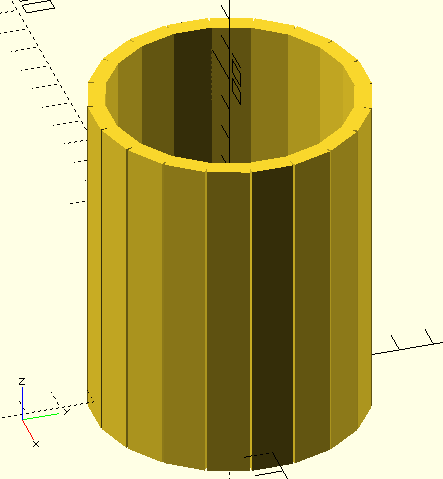
\includegraphics[width=.4\textwidth]{imagenes/torre-bug-1}  
  \caption{Los ladrillos de la flamante torre escrita por Cecilia no
    parecen apilarse como sería de desear.}
  \label{fig:torre-bug-1}
\end{figure}

---Nooo... ---gimió Cecilia, cubriendo sus ojos con una mano---. ¡No
me digas nada! ---atajó inmediatamente a An\-to\-\mbox{nia---.} Ya sé:
debo rotar los pisos para que cada ladrillo se apoye, por partes
iguales, en dos ladrillos del piso inferior. Toda torre que se precie
tiene que tener esa pinta.
    
Antonia asintió con una amplia sonrisa.

<<Muy bien, Cecilia, ¡A pensar!>> ---se dijo a sí misma,
  mientras volvía a sumergirse en su texto---. <<Cada piso,
    además de ser trasladado hacia arriba, debe ser rotado un cierto
    ángulo. Ahora bien, ¿cuánto vale ese ángulo?>> ---Cecilia se
  detuvo a pensar---. <<¡Pero si ya hice una cuenta muy parecida!
    Es la mitad del ángulo que abarca un ladrillo en su piso; éste era
    igual a $\frac{360^{\circ}}{\text{ladrillos\_por\_piso}}$; así que
    el ángulo que debo rotar un piso para que se `corra' como debe con
    respecto al anterior es
    $\frac{180^{\circ}}{\text{ladrillos\_por\_piso}}$>>.
  

%  \begin{center}
%  \begin{minipage}[t]{.55\textwidth}\vspace{0pt}
    \begin{lstlisting}
module torre(
  altura,
  n_pisos,
  radio,
  espesor,
  ladrillos_por_piso,
  factor_inter=.95) {
  alto_piso=altura/n_pisos;
  delta_alfa=180/ladrillos_por_piso;
  for (i=[0:n_pisos-1]){
   z=i*alto_piso;
   alfa=i*delta_alfa;
   rotate([0,0,alfa])
    translate([0,0,z])
      piso(radio=radio,
           espesor=espesor,
           altura=alto_piso,        
           n_ladrillos=ladrillos_por_piso,
           factor_inter=factor_inter);
  }
}    \end{lstlisting}
 %  \end{minipage}\hfill
%   \begin{minipage}[t]{.45\textwidth}\vspace{0pt}
%       \centering
%       \includegraphics[width=3cm]{vacio}
%     \end{minipage}
%
%   \end{center}

Cecilia volvió a releer sus últimas modificaciones al texto: en la
línea 9 definía la variable \lstinline!delta_alfa! de acuerdo a la
fórmula que dedujo momentos antes. Luego, en la línea 12, calculaba la
variable \lstinline!alfa!, con la que en la siguiente línea rotaba el
piso correspondiente dicho ángulo. Le pareció lógico: cada piso debía
ser rotado \lstinline!delta_alfa! grados con respecto al anterior, por
lo que las rotaciones se iban `acumulando': multiplicar \texttt{i} (el
número de piso) por \lstinline!delta_alfa! parecía la solución idónea.

  Instintivamente miró a Antonia para descubrir en su gesto algún otro
  error que se le hubiera pasado por alto, pero la encontró con una
  sonrisa impenetrable. Decidió entonces jugársela:

\begin{lstlisting}
torre(
 altura=100,
 radio=40,
 espesor=5,
 n_pisos=10,
 ladrillos_por_piso=20);
\end{lstlisting}%
\begin{figure}[ht]
  \centering
  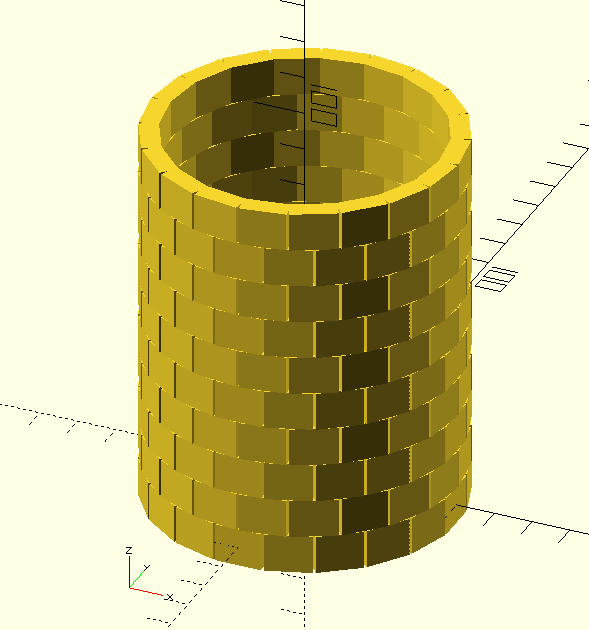
\includegraphics[width=.55\textwidth]{imagenes/torre-2}  
  \caption{La torre finalmente conquistada.}
  \label{fig:torre-2}
\end{figure}

  ¡Anduvo! ¡Por fin!

  Cecilia y Antonia se miraron con alarma: ¿quién había dicho
  eso?\footnote{Pido disculpas al lector: fui yo, naturalmente. El
    entusiasmo, usted entiende. Pero no le diga nada a
    ellas. Gracias.}

  \iftoggle{libro}{\vfill}{}

  \section{El texto completo, una apología y un poco de provocación}

  Cecilia y Antonia volvieron su atención al texto completo creador de torres.

    \begin{lstlisting}
module ladrillo (size) {
 cube(size,center=true) ;
}

module piso (
 radio,
 altura,
 espesor,
 n_ladrillos,
 factor_inter=0.95) {
  i_alfa=360/n_ladrillos;
  largo=2*PI*radio/n_ladrillos*factor_inter; 
  for (alfa=[0:i_alfa:359])
   rotate([0,0,alfa])
    translate([radio-espesor/2,0,0])
     ladrillo([espesor,largo,altura]); 
}

module torre (
  altura,
  n_pisos,
  radio,
  espesor,
  ladrillos_por_piso,
  factor_inter=.95) {
  alto_piso=altura/n_pisos;
  delta_alfa=180/ladrillos_por_piso;
  for (i=[0:n_pisos-1]){
   z=i*alto_piso;
   alfa=i*delta_alfa;
   rotate([0,0,alfa])
    translate([0,0,z])
      piso(radio=radio,
           espesor=espesor,
           altura=alto_piso,        
           n_ladrillos=ladrillos_por_piso,
           factor_inter=factor_inter);
  }
}
\end{lstlisting}

---¿Te das cuenta ahora de las posibilidades de crear objetos de forma
textual? ---los ojos de Antonia relampagueaban mientras con voz apenas
contenida comenzaba a confiar a Cecilia una de sus frecuentes
apologías---. Costó un poco de trabajo, eso sí; pero ahora podemos
crear todo tipo de torres con unas pocas líneas de texto:

    \begin{lstlisting}
torre(altura=100,
     radio=40,
     espesor=5,
     n_pisos=10,
     ladrillos_por_piso=20);
translate([100,0,0])
 torre(altura=150,
       radio=20,
       espesor=10,
       n_pisos=50,
       ladrillos_por_piso=20);
torre(altura=25,
       radio=150,
       espesor=8,
       n_pisos=5,
       ladrillos_por_piso=20);
\end{lstlisting}  



\begin{figure}[ht]
  \centering
  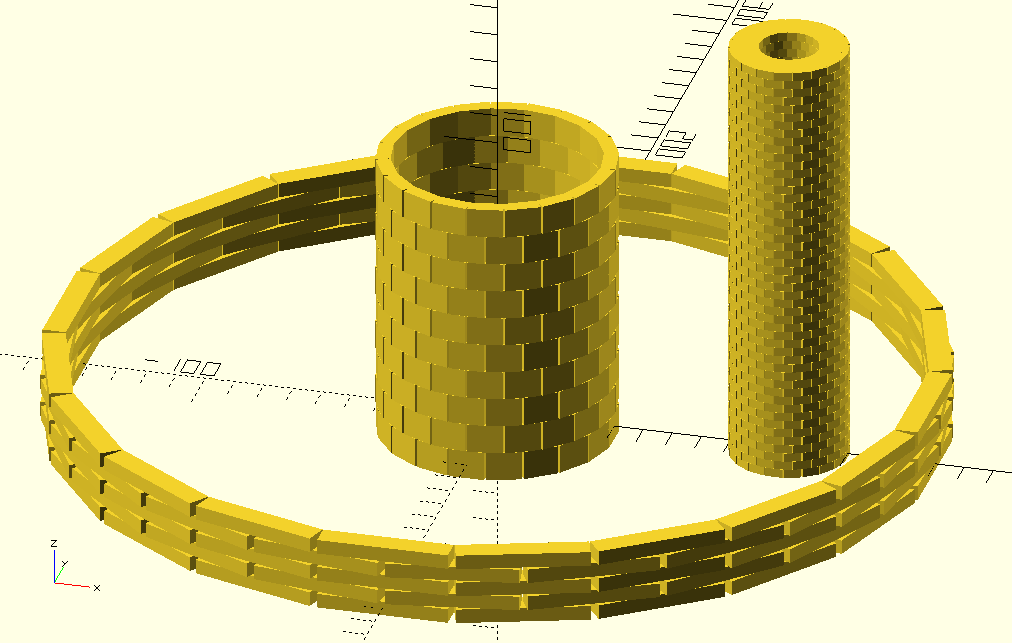
\includegraphics[width=.85\textwidth]{imagenes/torres}  
  \caption{Torres creadas por Antonia.}
  \label{fig:torres}
\end{figure}


\guillemotright Y no sólo eso: la posibilidad de crear tantas
variantes nos incita, tan sólo viéndolas, a realizar mejoras y
ampliaciones a lo ya conquistado: torres que no completen todo su
perímetro (`arcos' de torres, diríamos), torres que vayan aguzándose
hacia arriba, torres con almenas, torres con ladrillos faltantes... en
fin: ¡todas las posibilidades que sólo las palabras logran sugerir a
la imaginación!

Cecilia estaba casi convencida, pero rara vez podía acompañar a
Antonia en esos vuelos pretenciosamente retóricos.

---Además, decime la verdad ---el tono de Antonia se volvió
súbitamente confidencial---: ¿a vos te parece que esta variedad, fiel
a los delicados parámetros elegidos por el usuario, se puede lograr
con \emph{esos} programas que requieren el uso del ratón y los menúes
el 95\% del tiempo..?

Cecilia no podía sinceramente responder a esa pregunta; en todo caso,
tal comparación le parecía impertinente y al borde de la provocación. Le
pareció más productivo jugar un poco con sus torres:

\begin{lstlisting}
for(r=[10:50:200])
  torre(altura=200-r,
        radio=r,
        espesor=r*.2,
        n_pisos=(200-r)/10,
        ladrillos_por_piso=30);
\end{lstlisting}


\begin{figure}[ht]
  \centering
  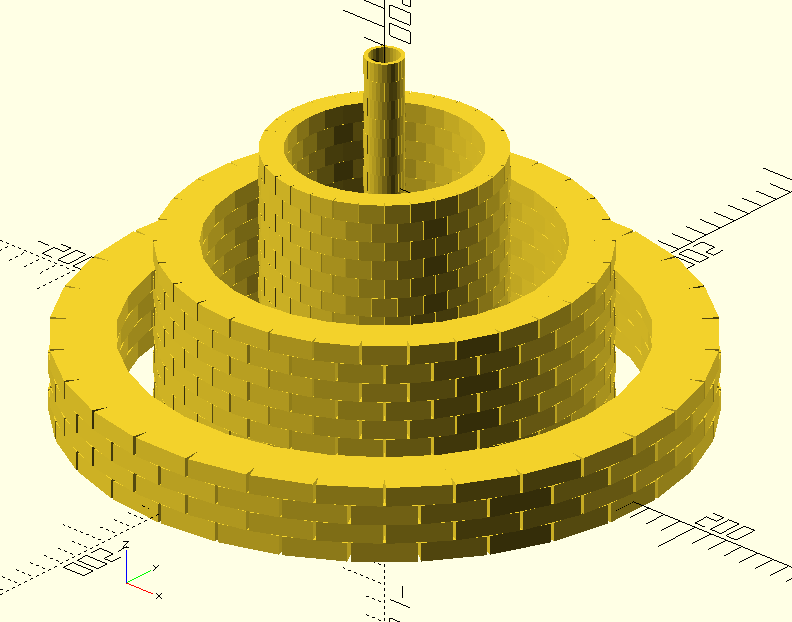
\includegraphics[width=.49\textwidth]{imagenes/torres-anidadas-1}\hfill
    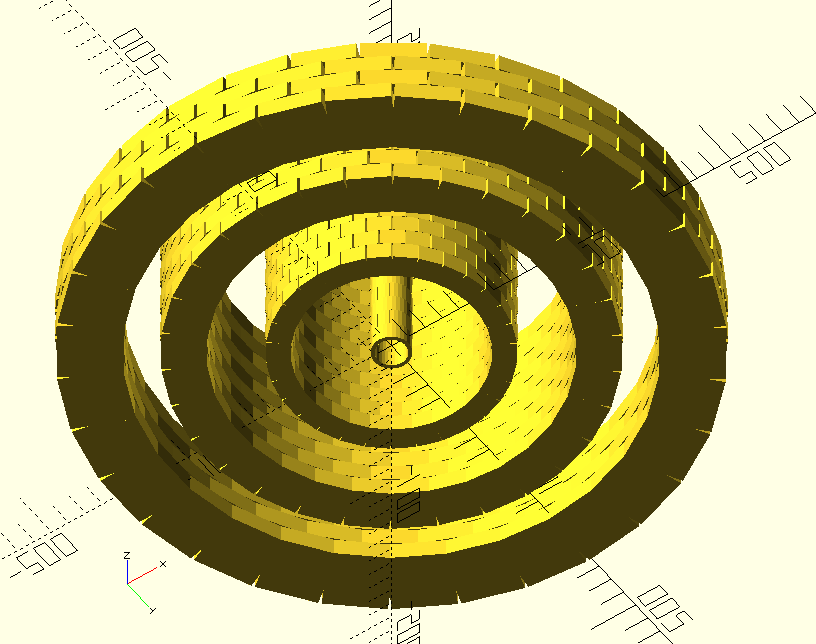
\includegraphics[width=.49\textwidth]{imagenes/torres-anidadas-2}    
    \caption{Torres anidadas con un bucle escritas por Cecilia.}
  \iftoggle{libro}{\vspace{128in}}{}
    \label{fig:torres-anidadas}
  \end{figure}


%%% Local Variables:
%%% mode: latex
%%% TeX-master: "../libro"
%%% End:
